\PassOptionsToPackage{unicode}{hyperref}
\PassOptionsToPackage{naturalnames}{hyperref}
\documentclass{article}
\usepackage{geometry}
%\usepackage{fullpage}
\usepackage{parskip}
\usepackage{physics}
\usepackage{amsmath}
\usepackage{amssymb}
\usepackage{xcolor}
\usepackage[colorlinks,linkcolor=blue,citecolor=green]{hyperref}
\usepackage{array}
\usepackage{longtable}
\usepackage{multirow}
\usepackage{comment}
\usepackage{graphicx}
\usepackage{cite}
\usepackage{amsfonts}
\usepackage{bm}
\usepackage{slashed}
\usepackage{dsfont}
\usepackage{mathtools}
\usepackage[compat=1.1.0]{tikz-feynman}
\usepackage{simplewick}
%\usepackage{fourier}
%\usepackage{slashbox}
%\usepackage{intent}
\usepackage{mathrsfs}
\usepackage{xparse}
\usepackage{enumerate}

\geometry{left=0.9cm,right=0.9cm,top=1.5cm,bottom=2cm}

\newcommand{\gm}{\gamma^{\mu}}
\newcommand{\gn}{\gamma^{\nu}}
\newcommand{\gs}{\gamma^{\sigma}}
\newcommand{\gr}{\gamma^{\rho}}
\newcommand{\gnr}{g^{\nu\rho}}
\newcommand{\gmr}{g^{\mu\rho}}
\newcommand{\gms}{g^{\mu\sigma}}
\newcommand{\gns}{g^{\nu\sigma}}
\newcommand{\vbp}{\vb{p}}
\newcommand{\vbk}{\vb{k}}
\newcommand{\g}{\gamma}
\renewcommand{\a}{\alpha}
\renewcommand{\b}{\beta}
\renewcommand{\t}{\theta}
\newcommand{\la}{\lambda}
\newcommand{\p}{\phi}
\newcommand{\vp}{\varphi}
\newcommand{\s}{\sigma}
\renewcommand{\G}{\Gamma}
\newcommand{\pars}{\slashed\partial}
\newcommand{\ps}{\slashed p}
\newcommand{\ks}{\slashed k}
\newcommand{\lag}{\mathcal{L}}

\title{Homework: Gauge Field Theory \#1}
\author{Yingsheng Huang}
\begin{document}
\maketitle
\begin{enumerate}[\bf 1.]
  \item $\phi^4$ theory ($\lag_I=\frac{\la}{4!}\phi^4$). Verify optical theorem in the lowest order.
$$\feynmandiagram[horizontal=x to y,baseline=(x.base)]{
	  i1 -- x -- f1,
	  i2 -- y -- f2,
	  x --[draw=none] y,
	  x --[quarter left,momentum=p-k] y,
	  x --[quarter right,momentum=k] y,
	};=\frac{(-i\la)^2}{2}\int\frac{\dd^4k}{(2\pi)^4}\frac{i}{k^2-m^2+i\epsilon}\frac{i}{(p-k)^2-m^2+i\epsilon}$$
For simplicity, we ignore the mass term.
$$i\mathcal{M}_2=\frac{(-i\la)^2}{2}\int\frac{\dd^4k}{(2\pi)^4}\frac{1}{k^2(p-k)^2}$$
Apply feynman parameterization
\begin{align*}
 i\mathcal{M}_2&=\frac{(-i\la)^2}{2}\int_0^1\dd x\int\frac{\dd^4k}{(2\pi)^4}\frac{1}{[x(p-k)^2+(1-x)k^2]^2}\\\intertext{$k\rightarrow k+xp$}
  &=\frac{(-i\la)^2}{2}\int_0^1\dd x\int\frac{\dd^4k}{(2\pi)^4}\frac{1}{[k^2+x(1-x)p^2+i\epsilon]^2}
\end{align*}
Set $\Delta\equiv -x(1-x)p^2+i\epsilon$, and apply wick rotation
$$i\mathcal{M}_2=\frac{i(-i\la)^2}{2}\int_0^1\dd x\int \frac{\dd^4k_E}{(2\pi)^4}\frac{1}{[k_E^2+\Delta]^2}$$
Dimensional regularization
\begin{align*}
  i\mathcal{M}_2&=\frac{i(-i\la)^2}{2}\int_0^1\dd x\int \frac{\dd^dk_E}{(2\pi)^d}\frac{1}{[k_E^2+\Delta]^2}\\
  &=\frac{i(-i\la)^2}{2}\int_0^1\dd x\int \frac{\dd\Omega_d}{(2\pi)^d}\dd k_E\frac{k_E^{d-1}}{[k_E^2+\Delta]^2}\\
  &=\frac{i(-i\la)^2}{2}\int_0^1\dd x\frac{\pi^{d/2}\G(2-d/2)}{\G(2)(2\pi)^d}\Delta^{d/2-2}\\
  &\xrightarrow{d\rightarrow4}-i\la^2\frac{\frac{2}{\epsilon}-\g+\mathcal{O}(\epsilon)}{32\pi^2}\int_0^1\dd x(\frac{\Delta}{4\pi})^{-\epsilon/2}\\
  &=-i\la^2\frac{\frac{2}{\epsilon}-\g+\mathcal{O}(\epsilon)}{32\pi^2}\int_0^1\dd x(1-\frac{\epsilon}{2}\ln{\frac{\Delta}{4\pi}})\\
  &=\frac{-i\la^2}{32\pi^2}(\frac{2}{\epsilon}-\g+2-\ln(-p^2)+\ln(4\pi)+\mathcal{O}(\epsilon))
\end{align*}
where $\epsilon=4-d$.

So
$$i\mathcal{M}(s)=-i\la+\frac{-i\la^2}{32\pi^2}(\frac{2}{\epsilon}-\g+2-\ln(-s)+\ln(4\pi))$$
$$\mathcal{M}(s)=-\la-\frac{\la^2}{32\pi^2}(\frac{2}{\epsilon}-\g+2-\ln(-s)+\ln(4\pi))=-\la-\frac{\la^2}{32\pi^2}(\frac{2}{\epsilon}-\ln(-s)+finite\ terms)$$
where $finite\ terms=\ln(4\pi)+2-\g$.
%\frac{\la_R-\la}{\la}=\frac{-\mathcal{M}(s_0)}{\la}-1$$
$$\la_R=\la+\frac{\la^2}{32\pi^2}(\frac{2}{\epsilon}-\ln(-s_0)+finite\ terms)$$
$$\la=\la_R-\frac{\la_R^2}{32\pi^2}(\frac{2}{\epsilon}-\ln(-s_0)+finite\ terms)$$
\begin{align*}
  \mathcal{M}(s)&=-\la-\frac{\lambda^2}{32\pi^2}(\frac{2}{\epsilon}-\ln{(-s)}+finite\ terms)\\
  &=-\la_R+\frac{\la_R^2}{32\pi^2}(\frac{2}{\epsilon}-\ln{(-s_0)}+finite\ terms)-\frac{\lambda_R^2}{32\pi^2}(\frac{2}{\epsilon}-\ln{(-s)}+finite\ terms)\\
  &=-\la_R-\frac{\la_R^2}{32\pi^2}\ln{\frac{s_0}{s}}
\end{align*}
As the lowest order, the results are always $-\la$.

Optical theorem concludes that 
$$\frac{\la^2}{16\pi}=\int\dd\Pi\la^2$$
where
\begin{align*}
  \int\dd\Pi\la^2&=\int\frac{\dd^3p_1\dd^3p_2}{(2\pi)^64E_1E_2}(2\pi)^4\delta^4(p-p_1-p_2)\la^2\\
  &=\frac{1}{16\pi}\la^2
\end{align*}

  \item Proca field, QED with massive photon. Calculate the leading order of $e^-e^-\rightarrow e^-e^-$.

	The propagator
	$$\mel{0}{T\{A_{in}^{\mu}(x)A_{in}^{\nu}(y)\}}{0}=\int\frac{\dd^4k}{(2\pi)^4}e^{-ik\cdot (x-y)}\frac{i(-g^{\mu\nu}+\frac{k^{\mu}k^{\nu}}{\mu^2})}{k^2-\mu^2+i\epsilon}+\frac{i}{\mu^2}\delta^4(x-y)\delta^{\mu0}\delta^{\nu0}$$

The Lagarangian is 
$$\lag=-\frac{1}{4}F^{\mu\nu}F_{\mu\nu}+\frac{1}{2}\mu^2A^{\mu}A_{\mu}+\bar\psi(i\slashed D-m)\psi$$
and the interaction part
$$\lag_I=e\bar\psi\gm\psi A_{\mu}$$
($\lag=-\frac{1}{4}F^{\mu\nu}F_{\mu\nu}+\frac{1}{2}\mu^2A^{\mu}A_{\mu}+\bar\psi(i\slashed \partial-m)\psi+e\bar\psi\gm\psi A_{\mu}$). The corresponding Hamiltonian is 
$$\mathcal{H}_I=A^{\mu}J_{\mu}+\frac{1}{2\mu^2}J_0^2=-e\bar\psi\gm\psi A_{\mu}+\frac{e^2}{2{\mu^2}}\bar\psi\g^0\psi\bar\psi\g_0\psi$$
and we have the propagator
\begin{align*}
  \mel{0}{T\{A_{\mu}(x)A_{\nu}(y)\}}{0}=\int\frac{\dd^4k}{(2\pi)^4}e^{-ik\cdot(x-y)}\frac{i(-g_{\mu\nu}+\frac{k_{\mu}k_{\nu}}{\mu^2})}{k^2-{\mu^2}+i\epsilon}+\frac{i}{{\mu^2}}\delta^4(x-y)\delta_{\mu}^0\delta_{\nu}^0
\end{align*}
and 
\begin{align*}
  \mel{k_1k_2}{T\{-i\mathcal{H}_I\}}{p_1p_2}&=i\mel{k_1k_2}{T\{e\bar\psi\gm\psi A_{\mu}-\frac{e^2}{2\mu^2}\bar\psi\g^0\psi\bar\psi\g_0\psi\}}{p_1p_2}
\end{align*}
At tree level(to $e^2$ order), the first part must be
\begin{align*}
  -e^2\mel{k_1k_2}{T\{\bar\psi\gm\psi A_{\mu}\bar\psi\gn\psi A_{\nu}\}}{p_1p_2}&
\end{align*}
so generally we have two diagrams
\begin{align*}
  \feynmandiagram[horizontal=x to y,baseline=(x.base)]{
	f1 --[fermion]y --[fermion]i1,
	f2 --[fermion]x --[fermion]i2,
	x--[photon]y,
  };\text{and}
  \feynmandiagram[horizontal=f2 to f1,baseline=(x.base)]{
	f1 --[anti fermion]x[blob] --[anti fermion]i1,
	f2 --[anti fermion]x --[anti fermion]i2,
	f1 --[draw=none]f2,
	i1 --[draw=none]i2,
  };
\end{align*}
with some exchange in external legs.

The contribution of the first one is 
\begin{align*}
  -\frac{1}{e^2}i\mathcal{M}_1=&\feynmandiagram[horizontal=x to y,baseline=(x.base)]{
	f1 --[fermion]y --[fermion]i1,
	f2 --[fermion]x --[fermion]i2,
	x--[photon]y,
  };+
  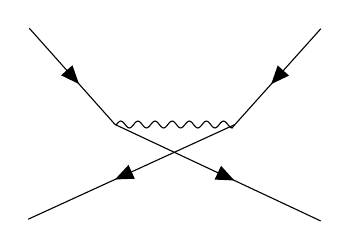
\begin{tikzpicture}[baseline=(x.base)]
	\begin{feynman}
	  \diagram[horizontal=x to y]{
	    f1 --[fermion]y --[draw=none]i1,
	    f2 --[fermion]x --[draw=none]i2,
	    x--[photon]y,
      };
	  \diagram*{
		(i1) --[anti fermion](x),
		(i2) --[anti fermion](y),
	  };
	\end{feynman}
  \end{tikzpicture}\\
  =&\bar u(k_1)\gm u(p_1)[\frac{i(-g_{\mu\nu}+\frac{k_{\mu}k_{\nu}}{\mu^2})}{k^2-{\mu^2}+i\epsilon}+\frac{i}{{\mu^2}}\delta_{\mu}^0\delta_{\nu}^0]\bar u(k_2)\gn u(p_2)
  -\bar u(k_2)\gm u(p_1)[\frac{i(-g_{\mu\nu}+\frac{k_{\mu}k_{\nu}}{\mu^2})}{k^2-{\mu^2}+i\epsilon}+\frac{i}{{\mu^2}}\delta_{\mu}^0\delta_{\nu}^0]\bar u(k_1)\gn u(p_2)\\
  =&\bar u(k_1)\gm u(p_1)[\frac{i(-g_{\mu\nu}+\frac{k_{\mu}k_{\nu}}{\mu^2})}{k^2-{\mu^2}+i\epsilon}]\bar u(k_2)\gn u(p_2)
  -\bar u(k_2)\gm u(p_1)[\frac{i(-g_{\mu\nu}+\frac{k_{\mu}k_{\nu}}{\mu^2})}{k^2-{\mu^2}+i\epsilon}]\bar u(k_1)\gn u(p_2)\\
  &+\frac{i}{\mu^2}\bar u(k_1)\g^0 u(p_1)\bar u(k_2)\g^0 u(p_2)
  -\frac{i}{\mu^2}\bar u(k_2)\g^0 u(p_1)\bar u(k_1)\g^0 u(p_2)
\end{align*}
and the second one is 
\begin{align*}
  i\mathcal{M}_2=&\frac{ie^2}{\mu^2}(\bar u(k_1)\g^0 u(p_1)\bar u(k_2)\g^0 u(p_2)-\bar u(k_2)\g^0 u(p_1)\bar u(k_1)\g^0 u(p_2))
\end{align*}
Combine these two and the incovariant terms are automatically canceled.

\item Vacuum polarization of massive photon.













\end{enumerate}




\end{document}

